\let\negmedspace\undefined
\let\negthickspace\undefined
\documentclass[journal]{IEEEtran}
\usepackage[a5paper, margin=10mm, onecolumn]{geometry}
%\usepackage{lmodern} 
\usepackage{tfrupee} 

\setlength{\headheight}{1cm} 
\setlength{\headsep}{0mm}     

\usepackage{gvv-book}
\usepackage{gvv}
\usepackage{cite}
\usepackage{amsmath,amssymb,amsfonts,amsthm}
\usepackage{algorithmic}
\usepackage{graphicx}
\usepackage{textcomp}
\usepackage{xcolor}
\usepackage{txfonts}
\usepackage{listings}
\usepackage{enumitem}
\usepackage{mathtools}
\usepackage{gensymb}
\usepackage{comment}
\usepackage[breaklinks=true]{hyperref}
\usepackage{tkz-euclide} 
\usepackage{listings}                                        
\def\inputGnumericTable{}                                 
\usepackage[latin1]{inputenc}                                
\usepackage{color}                                            
\usepackage{array}                                            
\usepackage{longtable}                                       
\usepackage{calc}                                             
\usepackage{multirow}                                         
\usepackage{hhline}                                           
\usepackage{ifthen}                                           
\usepackage{lscape}
\usepackage{caption}
\begin{document}

\bibliographystyle{IEEEtran}
\vspace{3cm}

\title{2.10.20}
\author{AI25BTECH11030 -Sarvesh Tamgade}
{\let\newpage\relax\maketitle}

\renewcommand{\thefigure}{\theenumi}
\renewcommand{\thetable}{\theenumi}
\setlength{\intextsep}{10pt} 


\numberwithin{equation}{enumi}
\numberwithin{figure}{enumi}
\renewcommand{\thetable}{\theenumi}


\textbf{Question}:  Which of the following expressions are meaningful?
\begin{multicols}{2}
\begin{enumerate}[label=(\alph*)]
     
\item $\vec{u} \cdot (\vec{v} \times \vec{w})$
\item $(\vec{u} \cdot \vec{v}) \cdot \vec{w}$
\item $(\vec{u} \cdot \vec{v})\ \vec{w}$
\item $\vec{u} \times (\vec{v} \cdot \vec{w})$

\end{enumerate}
\end{multicols}

\textbf{Solution}:\\
Let
\begin{align}
    \vec{u} &= \myvec{2 \\ 3}, \quad
    \vec{v} = \myvec{4 \\ 1}, \quad
    \vec{w} = \myvec{0 \\ 5}.
\end{align}

\begin{enumerate}[label=\alph*)]
  \item \( \vec{u}^\top (\vec{v} \times \vec{w}) \)
  
\[
\vec{v} \times \vec{w} =
\myvec{
v_{23} & w_{23} \\
v_{31} & w_{31} \\
v_{12} & w_{12}
}
=
\myvec{
v_2 w_3 - v_3 w_2 \\
v_3 w_1 - v_1 w_3 \\
v_1 w_2 - v_2 w_1
}
=
\myvec{
1 \times 0 - 0 \times 5 \\
0 \times 0 - 4 \times 0 \\
4 \times 5 - 1 \times 0
}
=
\myvec{
0 \\
0 \\
20
}
\]

\[
\vec{u}^\top (\vec{v} \times \vec{w}) =
\myvec{2 & 3 & 0}  % row vector (transpose of u)
\myvec{
0 \\
0 \\
20
}
= 0
\]

Since the scalar (dot) product of two vectors is defined, the expression  \(\vec{u}^\top(\vec{v} \times \vec{w})\) is meaningful.

  \item \( (\vec{u}^\top \vec{v})^\top \vec{w} \)

  \begin{align*}
  \vec{u}^\top \vec{v} &= \myvec{2 & 3} \myvec{4 \\ 1} = 2 \times 4 + 3 \times 1 = 11,
  \\
  (\vec{u}^\top \vec{v})^\top \vec{w} &= 11^\top \myvec{0 \\ 5} \quad \text{(scalar dot vector -- undefined)}.
  \end{align*}

  \item \( (\vec{u}^\top \vec{v}) \vec{w} \)
  
  \begin{align*}
  (\vec{u}^\top \vec{v}) \vec{w} &= 11 \times \myvec{0 \\ 5} = \myvec{0 \\ 55}.
  \end{align*}
  
  This is meaningful scalar multiplication.

  \item \( \vec{u} \times (\vec{v}^\top \vec{w}) \)
  
  \begin{align*}
  \vec{v}^\top \vec{w} &= \myvec{4 & 1} \myvec{0 \\ 5} = 0 + 5 = 5,
  \\
  \vec{u} \times 5 &= \text{cross product of vector and scalar -- undefined}.
  \end{align*}

\end{enumerate}

\textbf{Answer:}
\boxed{\text{Only (a) and (c) are meaningful }}
\begin{figure}[htbp]
    \centering
    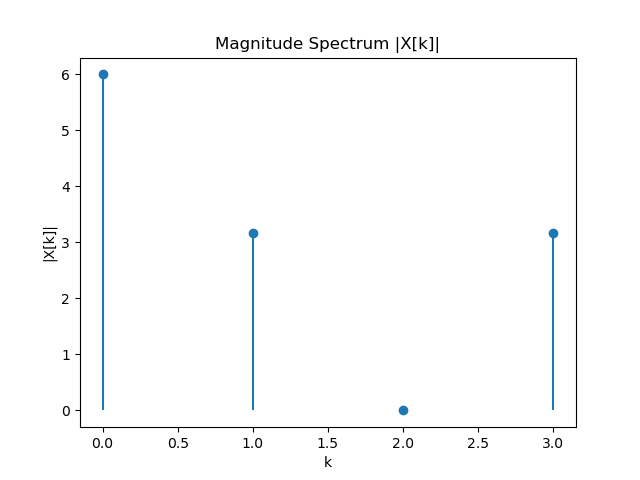
\includegraphics[width=0.65\linewidth]{FIG/fig1.png}
    \caption{Vector Representation}
    \label{fig:FIG/fig1.png}
    \end{figure}

\end{document}  